This interface was used to investigate the possible
route for experimental realization of laser plasma accelerator based coherent
light source (\glspl{fel})\cite{Emma2004}. \Glspl{lpa}~\cite{Leemans2006,Esarey2009,Tajima1979} have the potential to become the next
generation of accelerator facilities reaching field gradients of the order of
\SI{100}{\giga\electronvolt\per\metre}, i.e. up to three orders of magnitude
higher than in conventional linear accelerators. This would reduce construction
and operation costs by comparable orders of magnitude.

\subsection{Start--to--end simulation of \gls{lpa} based \glspl{fel}\label{sec:lwfa_s2e}}
Our simulation setup is shown in Fig.~\ref{fig:lwfa-setup}; starting from electron
beam generation from a laser plasma source to the generation of femtosecond
and/or attosecond EUV/XUV pulse from the radiation undulator.
%
\begin{figure}[ht]
  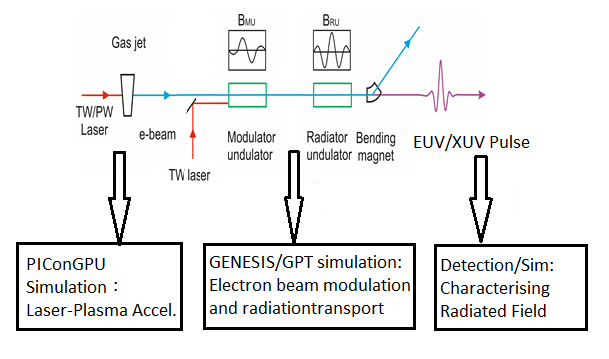
\includegraphics[width=5.4165in,height=2.7374in]{figures/lwfafel-img001.png}
  \caption{Scheme of \gls{lpa}--\gls{fel} simulation}
  \label{fig:lwfa-setup}
\end{figure}
%
In this scheme an intense
\SIrange{10}{100}{\tera\watt}
laser is focused onto a gas jet or a gas filled capillary for producing a
relativistic electron beam. Initial energy spread of the electron beam of a
\gls{lpa} (\numrange{1}{5}\%) is typically much larger than that of a linear accelerator
(about \num{0.05}\%), so
reduction of the slice energy spread is necessary. The electron beam is sent
through a modulator undulator (MU) together with a TW--power laser beam, where
the interaction between the electrons, the magnetic field of the undulator and
the electromagnetic field of the laser introduces a periodic energy modulation
of the electrons. This energy modulation leads to the formation of nano--bunches
(ultrashort electron layers). The nano--bunched electron beam then passes through
a radiator undulator (RU) consisting of a single or a few periods and creates
EUV/XUV pulses.
%
The SIMEX setup (as shown in Fig.~\ref{fig:lwfa-setup}) for \gls{lpa} driven \gls{fel}
utilizes the \textit{PIConGPU} simulation code for electron beam generation using the \gls{lpa}
mechanism and further transportation of electron beam to \gls{fel} simulation code
\textit{GENESIS}. We show schematically SIMEX tools in
Fig.~\ref{fig:lwfa-simulation_loop}, in order to calculate the radiation field
from \gls{lpa} generated electron beam. We start by defining the initial laser--plasma
parameters and initial conditions in \textit{PIConGPU} code using \gls{lpa} scheme.
\textit{PIConGPU} computes the 6D electron beam distributions at rear
side of  plasma in vacuum. The obtained electron beam distribution is
transformed via python script to a readable data format (an input data file for
\textit{GENESIS}); which is required to study the electron beam dynamics through the
magnetic field distributions in \gls{fel} simulation code. The output data file from
\textit{GENESIS} can be further post--processed to calculate and visulaize the radiation
field.

An online tutorial, demonstrating how to use the simulation capabilities and
data format converters will be added to the \textit{simex\_platform} wiki pages
soon. Generation of production simulation data for a realistic case study
is currently hindered by the unavailability of sufficient computing resources.
In order to simulate SIMEX for LPA driven FEL; we need adequate computing resources to run PIConGPU simulations for generation of high quality electron beam; a necessary condition for FEL radiation. At the moment, available GPUs for computation are short in numbers; subsequently we are unable to present the data in this report. A
proposal for compute time at a high performance computing facility (e.g. within the
PRACE) network) is currently being prepared.
\begin{figure}[ht]
  \begin{center}%
    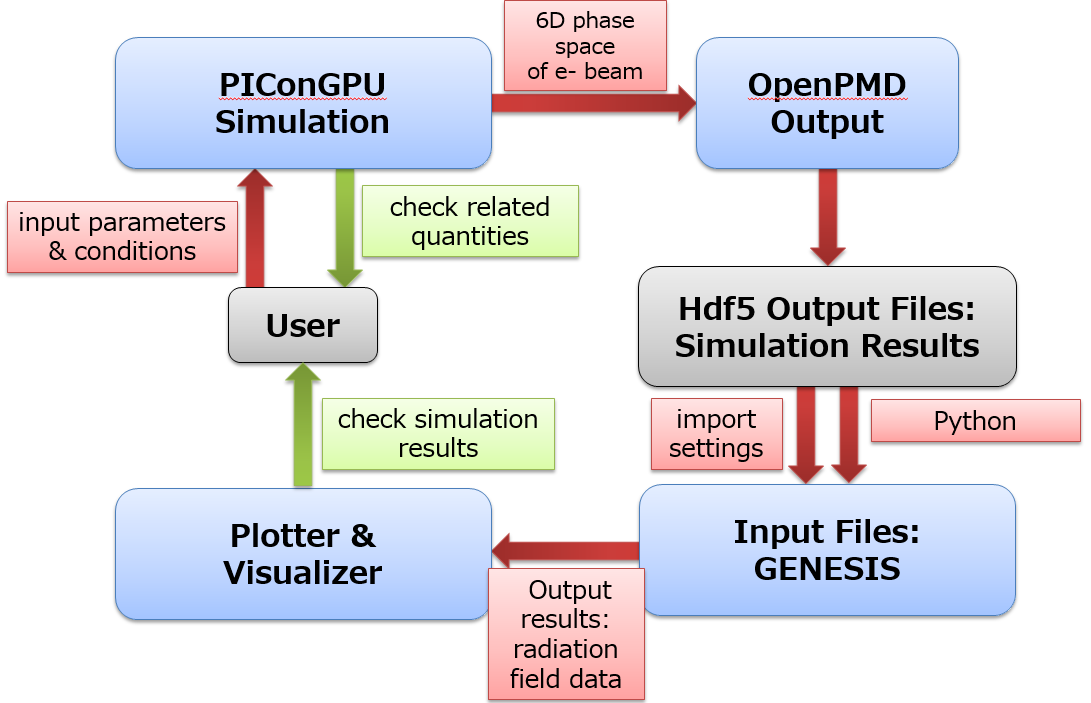
\includegraphics[width=5.9425in,height=4.1882in]{figures/lwfafel-img002.png}
    \caption{Layout for simulation setup and feedback loop}
    \label{fig:lwfa-simulation_loop}
  \end{center}%
\end{figure}
%
\subsection{Laser--plasma accelerator based single--cycle attosecond undulator source}
In parallel, we have studied\footnote{This study was performed in collaboration
with T. Zoltan and Prof. Hebling, both at Pecs University, Hungary.} the feasability of a \gls{lpa} based coherent light
source using experimental data for electron wakefield acceleration as input to
the \gls{fel} simulation. The \gls{fel} simulation used the code \textit{GPT} in this case.
Details are discussed in Ref.~\cite{Tibai2017}.

Fig.~\ref{fig:Tibai2017} displays the simulated waveform (electric field as
a function of time)  of the generated attosecond
pulse and the beam profile at \SI{60}{\nano\metre} radiation wavelength. The
temporal evolution was measured on the axis of highest intensity, marked by  a
cross in Fig.~\ref{fig:Tibai2017_profile}. In other
wavelengths the shape of the attosecond pulses are nearly identical with the
shape shown in Fig.~\ref{fig:Tibai2017_E_vs_t}, showing that these pulses are
\gls{cep} controlled \cite{Tibai2017}.
%
\begin{figure}[ht]
  \centering{%
    \subfloat[]{
      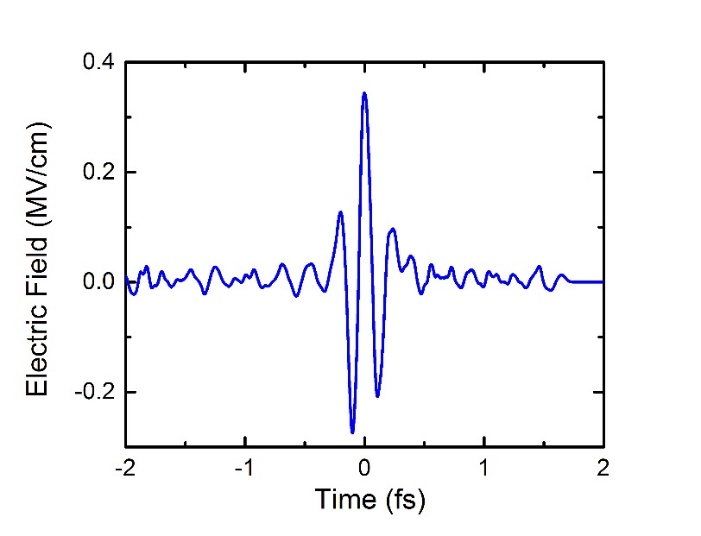
\includegraphics[width=2.7016in,height=2.1583in]{figures/lwfafel-img003.jpg}
      \label{fig:Tibai2017_E_vs_t}
    }
    \subfloat[]{
      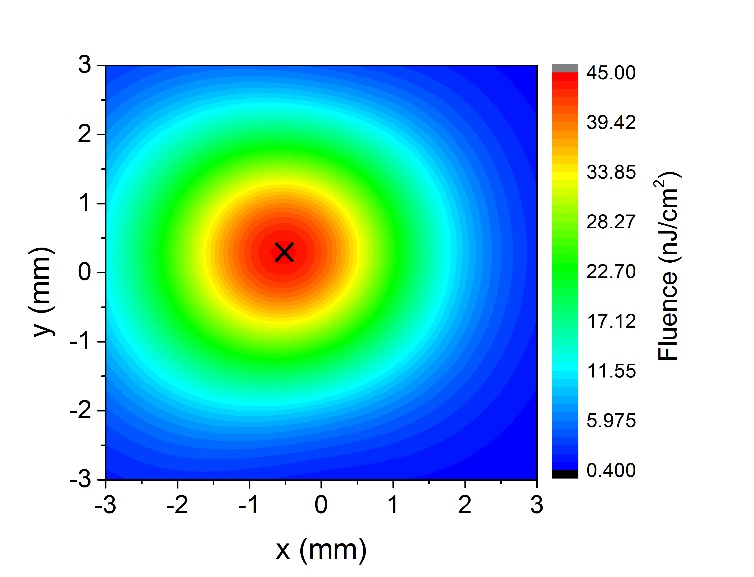
\includegraphics[width=3.0083in,height=2.352in]{figures/lwfafel-img004.jpg}
      \label{fig:Tibai2017_profile}
    }
  }
  \caption{GPT Simulation Results: \gls{cep}--controlled \gls{euv} waveforms (left) and its spatial beam
    profile (right).}
    \label{fig:Tibai2017}
\end{figure}

